\documentclass[11pt,aspectratio=169]{beamer}

\usepackage{amssymb}

\title{Torus amplitudes and modular invariance}
\date[16.5.2022]{Seminar on Theoretical Physics}
\author{Otto T.P. Schmidt}
%\institute[Organizational Unit]{Organizational Unit\\can spread over 2 lines}
\institute[Department of Physics]{}
\usetheme{eth}

\colorlet{titlefgcolor}{ETHblue}
\colorlet{accentcolor}{ETHred}

\begin{document}

%\def\titlefigure{elements/title-page-image}		% Default image
%\def\titlefigure{elements/title-page-image-43}	% Use this for 4:3 presentations

\titleframe

% \colorlet{titlefgcolor}{ETHpurple}
% \def\titlefigure{elements/title-page-image-alt}
% \title{Different background}
% \titleframe

% \colorlet{titlefgcolor}{ETHgreen}
% \colorlet{titlebgcolor}{ETHgreen!60!black}
% \def\titlefigure{}
% \setlength{\titleboxwidth}{0.75\textwidth}			% Change box width
% \title{Or even a plain color, especially if your title is very long and leaves no space for what's behind the colored box}
% \titleframe

\tocframe

\section{Motivation}

\begin{frame}[fragile]{Interactions and observables}

	In the study of string interactions, the ultimate goal will be the assignment of a probability for a certain process and the prediction of a physical cross section.
	\\~\\
	As outlined in Section 22, the computation of an observable cross section involves a series of steps:
	\begin{enumerate}
		\item Canonical representation of string diagram through moduli space
		\item Compute scattering amplitude by means of conformal field theory
		\item Convert scattering amplitude into a cross section
	\end{enumerate}
	
	
		




\end{frame}

\begin{frame}[fragile]{Loop amplitudes in string theory}
	
	In order to obtain accurate scattering amplitudes of processes,
	one needs to include contributions from loops in string diagrams. 
	\\~\\
	These loops can be seen as contributions
	from the next higher order pertubation. 
	Graphically we consider the following processes:
	\begin{figure}[htbp]
		\centering
		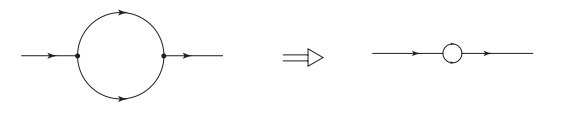
\includegraphics[width = 0.55\textwidth]{elements/Feynman loop}
	\end{figure}


\end{frame}

\begin{frame}{\underline{Ultraviolet divergence}}

	Amplitudes from virtual processes as depicted before can lead to ultraviolet (UV) divergences in quantum field theory (QFT).
	\\~\\
	Whereas QFT must employ complex renormalizations to deal with these UV divergences, we do not encounter these problems in string theory.
	
\end{frame}



\section{The moduli space of tori}

\begin{frame}[fragile]{\underline{One-loop open strings}}

	Before approaching the moduli space of tori, lets consider a one-loop open string with light-cone momentum $p^{+}$. This will serve as an intuitive analogon.

	The light-cone diagram is:
	\begin{figure}[htbp]
		\centering
		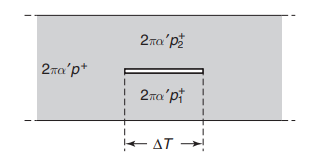
\includegraphics[width = 0.45\textwidth]{elements/one-loop open string.PNG}
	\end{figure}

	For fixed external momentum $p^+$ we find the two parameters: $\Delta T \in (0, \infty)$ and $p_{1}^{+} \in (0, p^+)$.
	\\
	$\rightarrow$ The class of Riemann surfaces of this process has two moduli.

\end{frame}

\begin{frame}{\underline{Canonical annulus}}

	Use $w = \tau + i \sigma$ and apply conformal transformations:
	\\~\\
	\begin{enumerate}
		\item Exponential map: $z = exp[\frac{w}{2 \alpha^{'} p^+}]$
		\item Linear fractional transformation: $\eta = \frac{1+iz}{1-iz}$
		% \item Canonical annulus: \textit{A region in} \mathbb{C} \textit{that is topologically an annulus can be mapped conformally to a canonical annulus}
		\item Canonical annulus: \textit{A region in $\mathbb{C}$ that is topologically an annulus can be mapped conformally to a canonical annulus}

	\end{enumerate}

	\begin{columns}
		\begin{column}{0.25\textwidth}
			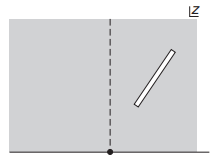
\includegraphics[width=\columnwidth]{elements/exponential map.PNG}
		\end{column}
		\begin{column}{0.25\textwidth}
			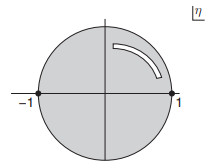
\includegraphics[width=\columnwidth]{elements/LFT.PNG}
		\end{column}
		\begin{column}{0.25\textwidth}
			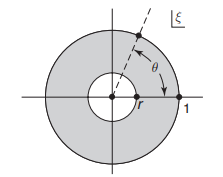
\includegraphics[width=\columnwidth]{elements/canonical annulus.PNG}
		\end{column}
	\end{columns}
	
\end{frame}

\begin{frame}{\underline{Rectangular torus}}

	In order to apply the concept of moduli spaces to a torus, we need to assure that a torus is indeed a Riemann surface.
	\\
	Consider a rectangular region of $\mathbb{C}$. By applying the analytic identifications $z \sim z + L_1$ and $z \sim z + iL_2$
	we obtain a torus. This shows that the region remains a Riemann surface. 
	\\
	Graphically:
	\begin{columns}
		\begin{column}{0.25\textwidth}
			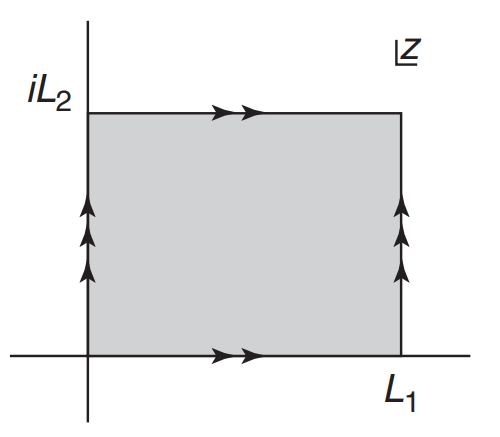
\includegraphics[width=\columnwidth]{elements/region C.PNG}
		\end{column}
		\begin{column}{0.2\textwidth}
			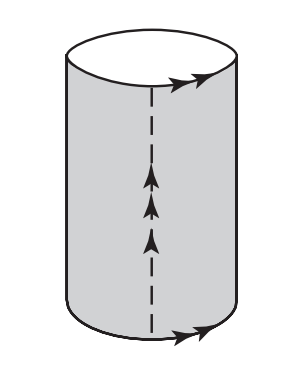
\includegraphics[width=\columnwidth]{elements/first ident.PNG}
		\end{column}
		\begin{column}{0.25\textwidth}
			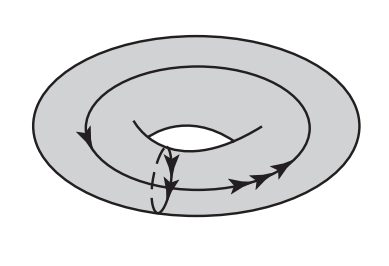
\includegraphics[width=\columnwidth]{elements/second ident.PNG}
		\end{column}
	\end{columns}


	
\end{frame}

\begin{frame}[fragile]{Colors}

	You need to pick these colors
	\begin{itemize}
		\item \texttt{titlefgcolor} (the box on the title page)
		\item \texttt{titlebgcolor} (the background on the title page, in case you don't use an image)
		\item \texttt{accentcolor} (alert text, blocks)
	\end{itemize}
	Use these commands at the beginning of the document
	\begin{verbatim}
		\colorlet{titlefgcolor}{ETHblue}
		\colorlet{titlebgcolor}{ETHblue!60!black}		% Use only multiples of 20%
		\colorlet{accentcolor}{ETHred}
	\end{verbatim}

	\medskip

	\begin{tabular}{ll}
	\textcolor{ETHblue}{\rule{4mm}{3mm}} ETHblue &
	\textcolor{ETHpetrol}{\rule{4mm}{3mm}} ETHpetrol \\
	\textcolor{ETHgreen}{\rule{4mm}{3mm}} ETHgreen &
	\textcolor{ETHbronze}{\rule{4mm}{3mm}} ETHbronze \\
	\textcolor{ETHred}{\rule{4mm}{3mm}} ETHred &
	\textcolor{ETHpurple}{\rule{4mm}{3mm}} ETHpurple \\
	\textcolor{ETHgray}{\rule{4mm}{3mm}} ETHgray 
	\end{tabular}
	
	\medskip

	Old ETH colors (\verb+ETH1+, ..., \verb+ETH9+) are deprecated and should not be used.\\
	They are available as \verb+oldETH1+, ..., \verb+oldETH9+ for backward compatibility.
	

\end{frame}

\begin{frame}

	\frametitle{Title}
	\framesubtitle{Subtitle}
	
	Text and some \alert{alert text}
	
	\[
	m_a^\top h(\cdot)
	\]
	
	
	\begin{itemize}
	\item list one
	\item list another one
		\begin{itemize}
		\item test 1
		\item test 2
		\end{itemize}
	\end{itemize}

\end{frame}

\section{Torus partition function}

\begin{frame}{Title with no subtitle}

	\begin{block}{Large box}
	Notice that blocks are a bit larger than the text, that's intended.
	\end{block}
	
	Column environments also eat some margins. Use the option \texttt{[onlytextwidth]} if you want to align columns to the wide blocks.
	
	\begin{columns}[onlytextwidth]
	\begin{column}{0.45\textwidth}
		\begin{block}{Small box}
		With some more text
		\end{block}
	\end{column}
	\begin{column}{0.5\textwidth}
		Think outside the box!
	\end{column}
	\end{columns}

\end{frame}

\section{Modular invariance}

\begin{frame}{And, of course, figures!}
	
	\begin{columns}
		\begin{column}{0.33\textwidth}
			\includegraphics[width=\columnwidth]{example-image-a}
		\end{column}
		\begin{column}{0.33\textwidth}
			\includegraphics[width=\columnwidth]{example-image-b}
		\end{column}
		\begin{column}{0.33\textwidth}
			\includegraphics[width=\columnwidth]{example-image-c}
		\end{column}
	\end{columns}

\end{frame}

\begin{frame}[fragile,t]{Free overlay}

	The package \verb+textpos+ is also enabled in case you want to overlay content freely in the slide.

	\begin{textblock}{18}(1,3)
		{\tiny \color{accentcolor}
		This text is located at position (1,3):\\
		\verb+\begin{textblock}{3}(1,3) ... \end{textblock}+ \\
		(1 unit equals to the left text margin)\par}
	\end{textblock}

	\begin{textblock*}{60mm}(0.5\paperwidth,0.5\paperheight)
		{\tiny \color{accentcolor}
		\includegraphics[width=20mm]{example-image-a}\\[2mm]
		The upper left corner of this image is at the slide center point:\par
		\verb+\begin{textblock*}{40mm}(0.5\paperwidth,0.5\paperheight)+\par
		\verb+   \includegraphics[width=20mm]{example-image-a}+\par
		\verb+\end{textblock*}+\par }
	\end{textblock*}	

\end{frame}

\begin{frame}

	\frametitle{Tables}
	\framesubtitle{Don't use vanilla \LaTeX{}  tables please}
	
		\begin{center}
			\begin{tabular}{@{}llr@{}}
				\toprule\multicolumn{2}{c}{Item} \\
				\cmidrule(r){1-2}Animal & Description & Price (\$)\\
				\midrule
				Gnat  & per gram  & 13.65 \\
				& each      & 0.01 \\
				Gnu   & stuffed   & 92.50 \\
				Emu   & stuffed   & 33.33 \\
				Armadillo & frozen & 8.99 \\
				\bottomrule
			\end{tabular}
		\end{center}

\end{frame}

\section{URLs and links}

\begin{frame}{Clickable links}

	Lorem ipsum dolor sit amet, consectetur adipiscing elit, sed do eiusmod tempor incididunt ut labore et dolore magna aliqua. 
	Ut enim ad minim veniam, quis nostrud exercitation...
	
	\medskip

	\url{http://control.ee.ethz.ch}
	
	\href{http://control.ee.ethz.ch}{Automatic Control Laboratory}
	
	\email{name@ethz.ch}

\end{frame}

\begin{closingframe}

Professor John Doe\\
Role of person giving presentation\\
\email{beat.muster@abcd.ethz.ch}

\medskip

ETH Zurich\\
Organisational unit\\
Building Room\\
Street House number\\
0000 Town, Country\\
\url{http://www.abcd.ethz.ch}

\end{closingframe}


\begin{closingframe}

	You can edit the content of the \texttt{closingframe} environment to design your own closing frame. Example:
	
	\vspace{15mm}

	\begin{columns}
		\begin{column}{0.55\textwidth}
			\raggedleft
			
\includegraphics[width=40mm]{elements/ifa_logo} 
		\end{column}
		\begin{column}{0.45\textwidth}
			\textbf{Author name}\\
			\email{name@ethz.ch}	
		\end{column}
	\end{columns}

	\vspace{20mm}
			
\end{closingframe}


\end{document}